\section{Auswertung}
	Da unsere getemperte Probe ungewöhnlich viele Ätzgrübchen aufweist und im Verlauf des Versuchs beschädigt wurde, haben wir eine weitere getemperte Probe erhalten und somit insgesamt 3 Proben untersucht.
    \subsection{Ätzgrübchendichte}
        Zunächst gilt es, als eine erste Näherung der Versetzungsdichte die Ätzgrübchendichte an der Oberfläche zu bestimmen.
	Dazu wurden für beide Proben je 3 Bilder von verschiedenen Positionen an der Oberfläche aufgenommen und anschließend
        aus der Fläche, aufgenommen durch das Mikroskop, und den sichtbaren Ätzgrübchen die Ätzgrübchendichte bestimmt. Dieser Vorgang ist,
        durch das manuelle Zählen der Grübchen sehr müßig und ungenau, lässt aber dennoch eine Qualitative aussage über die Ordnung im Kristall zu.
        Aus den Aufgenommen Bildern lies sich folgende Tabelle erstellen.
        \begin{table}[H]
            \centering
            \begin{tabular}[]{c|c|c|c|c}
                Probe & Aufnahme Nr. & Anzahl Grübchen & Fläche [$\mu m^2$] & Dichte [$\frac{n}{\mu m^2}$] \\
                \hline
                \multirow{3}{*}{\rotatebox[origin=c]{90}{Get.}} & 1 & $39 \pm 3$ & 839908,67$\pm$0,01 & $(4,64\pm 0,37)\cdot 10^{-5}$ \\
                                                                     & 2 & $25 \pm 3$ & 1099357,61$\pm$0,01 & $(2,27\pm 0,28)\cdot 10^{-5}$ \\
                                                                     & 3 & $31 \pm 3$ & 454314,66$\pm$0,01 & $(6,82\pm 0,67)\cdot 10^{-5}$ \\
                Mittelwert                                           & - & - & - & $(4,6\pm 0,47)\cdot 10^{e-5}$\\
                \hline
                \multirow{3}{*}{\rotatebox[origin=c]{90}{Unget.}}  & 1 & $344 \pm 40$  & 18894,73$\pm$0,01 & $(1,82 \pm 0,21)\cdot 10^{-2}$ \\
                                                                        & 2 & $27 \pm 5$    & 7942,73$\pm$0,01 & $(0,34\pm 0,06)\cdot 10^{-2}$ \\
                                                                        & 3 & $103 \pm 15$  & 6251,25$\pm$0,01 & $(1,74e\pm 0,24)\cdot 10^{-2}$ \\
                Mittelwert                                           & - & - & - & $(1,27 \pm 0,19)\cdot 10^{-2}$\\
                
            \end{tabular}    
        \end{table}
	Als Flächenfehler nehmen wir an, dass aus der angegebenen Genauigkeit des Auswertungsprogramms ein Fehler von 0,1 $\mu m^2$ resultiert.
	Der Fehler der Dichte ergibt sich gemäß Fortpflanzung zu $\Delta \rho = \sqrt{(\frac{\Delta n}{A})^2 + (\frac{n\Delta A}{A^2})^2}$.
	Den Gesamtfehler des Mittelwerts bestimmen wir über $\Delta \rho^2 = (\sum_{i=1}^3 \Delta \rho_i^2)/3$, mit den drei Einzelfehlern $\rho_i$. Die Standardabweichung zum Mittelwert der getemperten Probe beträgt $2,27\cdot 10^{-2}$, der Standardfehler $1,31\cdot 10^{-5}$, diese Werte berücksichtigen jedoch keine Grübchenzahl- und Flächenfehler. Für die ungetemperte Probe ergeben sich eine Standardabweichung von $0,8\cdot 10^{-2}$ sowie ein Standardfehler von $0,5\cdot 10^{-2}$.\\
        Es ist deutlich zu erkennen, dass die Ätzgrübchendichte der ungetemperten Probe um ein Vielfaches höher ist, als die der getemperten.
        Auch ist zu erkennen, dass die Ätzgrübchendichte an verschiedenen stellen der Oberfläche stark variiert, also nicht konstant ist.
    \begin{figure}[H]
        \centering
        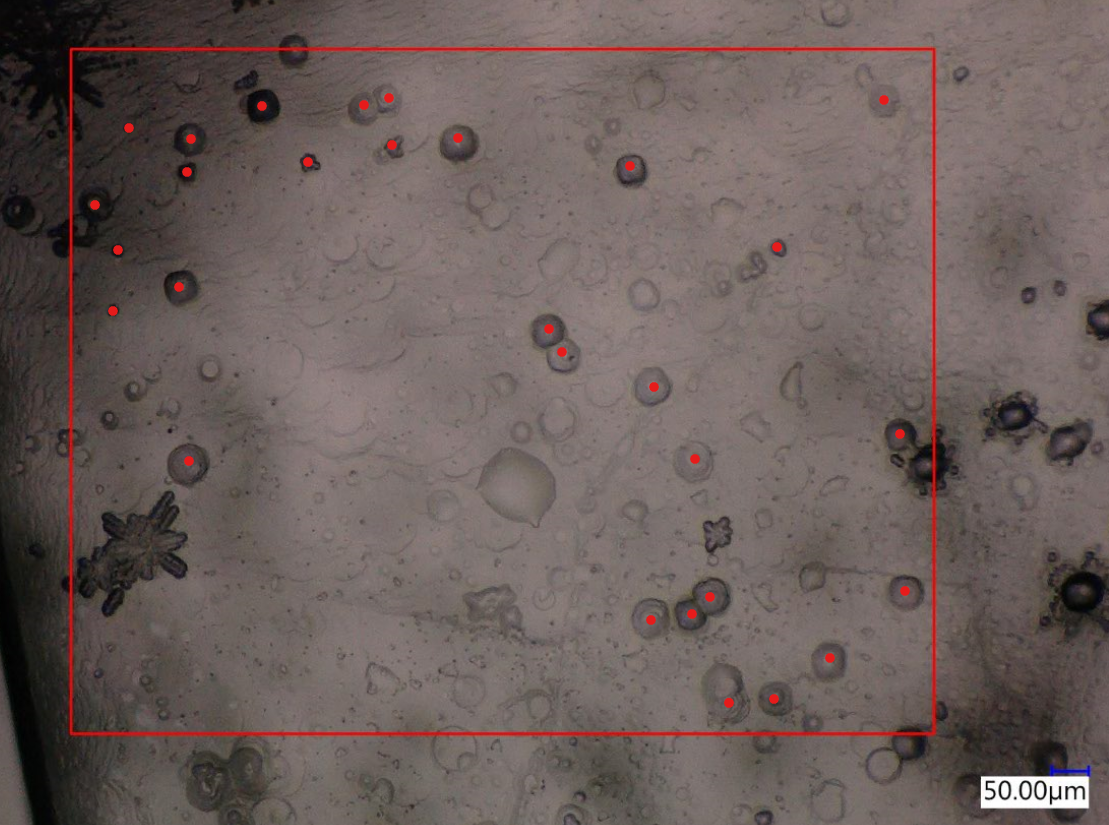
\includegraphics[width=\textwidth]{Images/Beispiel_ätzgrübchendichte.PNG}
        \caption{Beispiel einer Aufnahme für die Ätzgrübchendichte.}
    \end{figure}

    \subsection{Kleinwinkelkorngrenzen}
        \subsubsection*{Rosetten durch Nadeleindruck}
            Im Anschluss an die Bestimmung der Ätzgrübchendichte wurde auch ein Bild einer vermutlichen Kleinwinkelkorngrenzen aufgenommen, um aus diesem
            den Winkel zwischen den Kristalliten zu bestimmen. Um den Winkel aus den Abständen zwischen den Ätzgrübchen zu bestimmen wurde bereits in der Vorbereitung
            folgende Formel hergeleitet
            \begin{equation}
                \theta \approx \frac{b}{d} \approx \frac{(n-1)\cdot a}{\sqrt{2}\cdot d}
            \end{equation}
            Wobei $n$ die Anzahl der Ätzgrübchen angibt und $d$ den abstand zwischen dem ersten und letzten. Zudem nehmen wir für $b=\frac{a}{\sqrt{2}}$ an, sodass für
            Messungen mit mehreren Grübchen ein gesamt Verschiebung von $b_ges = n * g$ gilt.
            Mit folgender Aufnahme
            \begin{figure}[H]
                \centering
                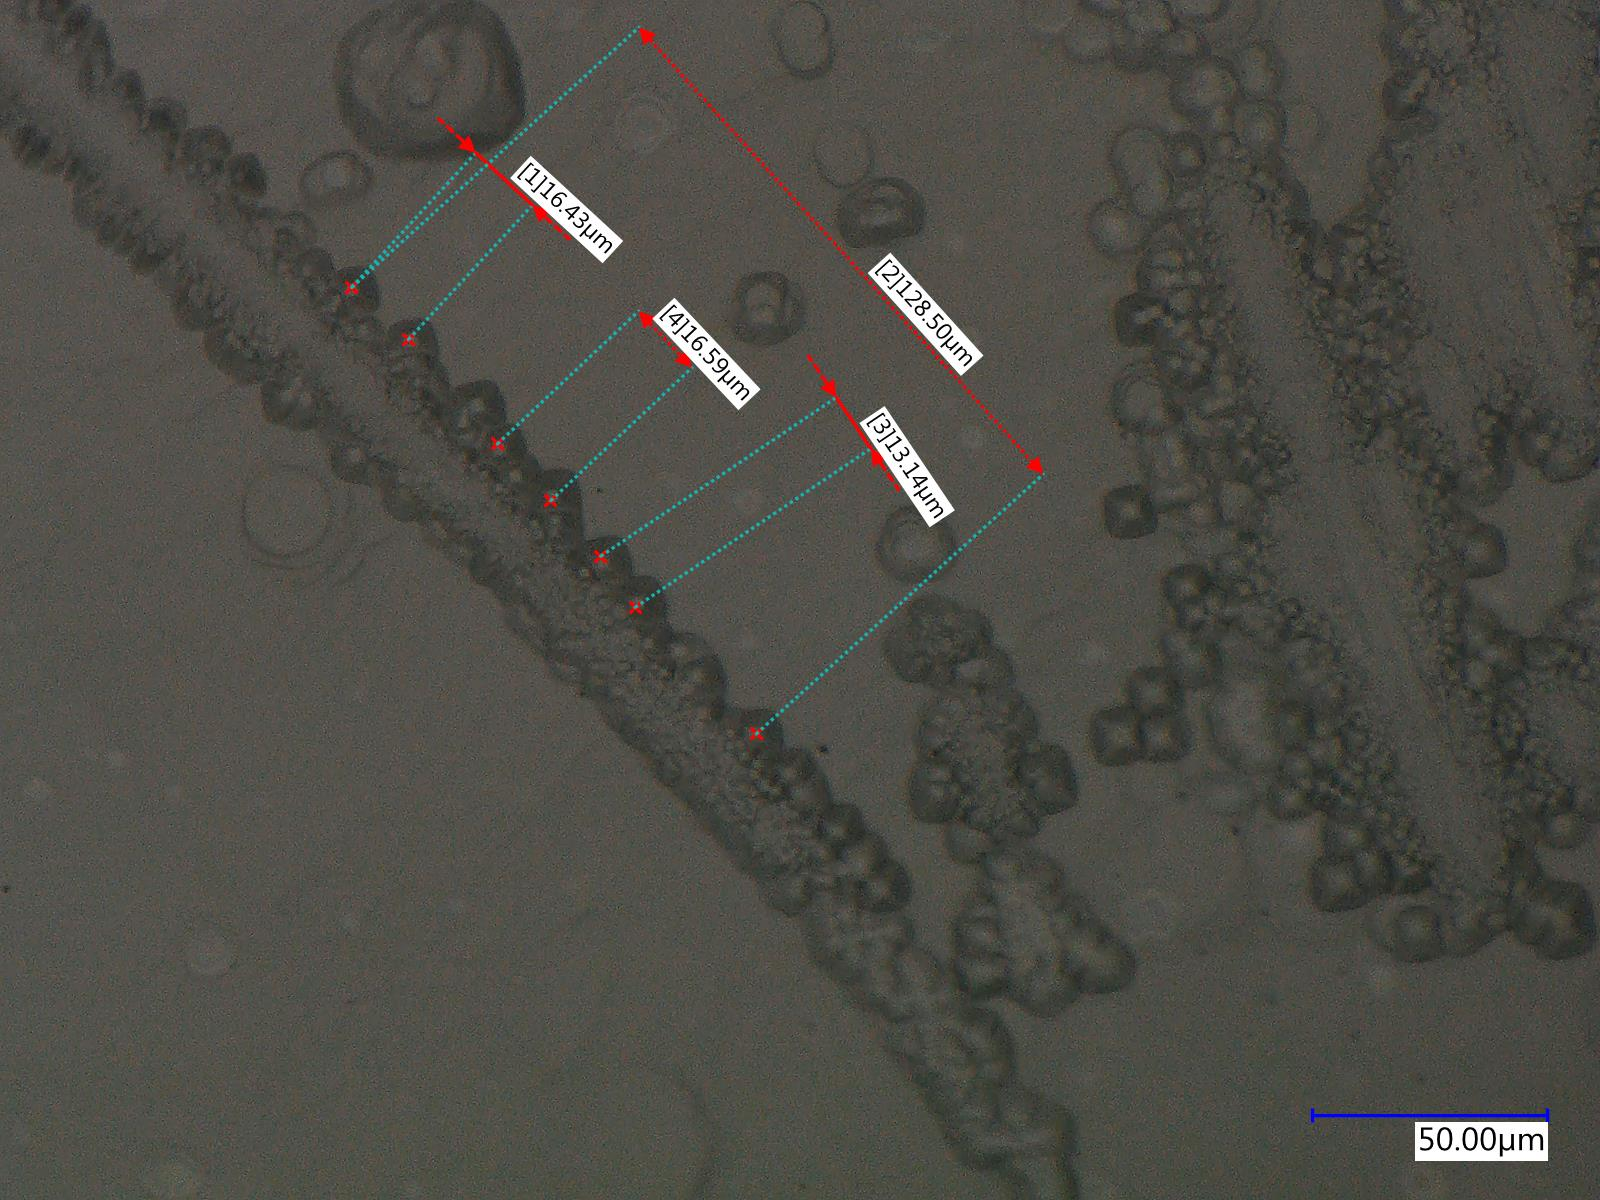
\includegraphics[width=\textwidth]{Images/kleinwinkelkorngrenze 2.jpg}
                \caption{Aufnahme einer vermutlichen Kleinwinkelkorngrenzen mit Abständen}
            \end{figure}
            konnte folgende Tabelle erstellt werden
            \begin{table}[H]
                \centering
                \begin{tabular}[]{c|c|c}
                    Abstand d [$\mu m$] & Anzahl Grübchen (n-1) & Winkel $\theta$ [°] \\
                    \hline
                    $128,5 \pm 0.1$ & 9 & $(1,14 \pm 0,0192)\cdot 10^{-3}$\\
                    $16,4 \pm 0.1$ & 1 & $(0,99 \pm 0,151)\cdot 10^{-3}$\\
                    $16,6 \pm 0.1$ & 2 & $(1,96 \pm 0,149)\cdot 10^{-3}$\\
                    $13,1 \pm 0.1$ & 1 & $(1,24 \pm 0,189)\cdot 10^{-3}$\\   
                \end{tabular}
            \end{table}
		Die jeweiligen Winkelfehler ergeben sich dabei durch Fehlerfortpflanzung aus $\Delta \theta = \frac{(n-1)\cdot a}{\theta\cdot d^2}\cdot \Delta d$.
            Grundsätzlich entsprechen die Winkel den Erwartungen, da diese recht klein ausfallen. Eine Kleinwinkelkorngrenze, die mehr auf einer Linie befindliche Ätzgrübchen erzeugt hätte,
		hätte jedoch eine genauere Winkelmessung ermöglicht.
% jedoch lässt die Messmethode nur ganzzahlige n zu, die nur eine geringe Auflösung der Tatsächlichen abstände d zulassen.
        \subsection{Versetzungsbewegungen}
            Dieser abschnitt befasst sich mit der Wanderung der Versetzungen bei äußerer Druckeinwirkung, dazu wurden 2-3 Rosetten durch Nadeleindruck erzeugt,
            deren Dimension über das Mikroskop aufgenommen und anschließend durch axialen Druck bewegt. Durch das Gewicht der Presse sowie der Querschnittsfläche der Probe
            lässt sich die Kraft bestimmen und über die Dauer der Anwendung die Geschwindigkeit der Wanderung.
            \begin{figure}[H]
                \begin{minipage}[b]{.4\linewidth} % [b] => Ausrichtung an \caption
                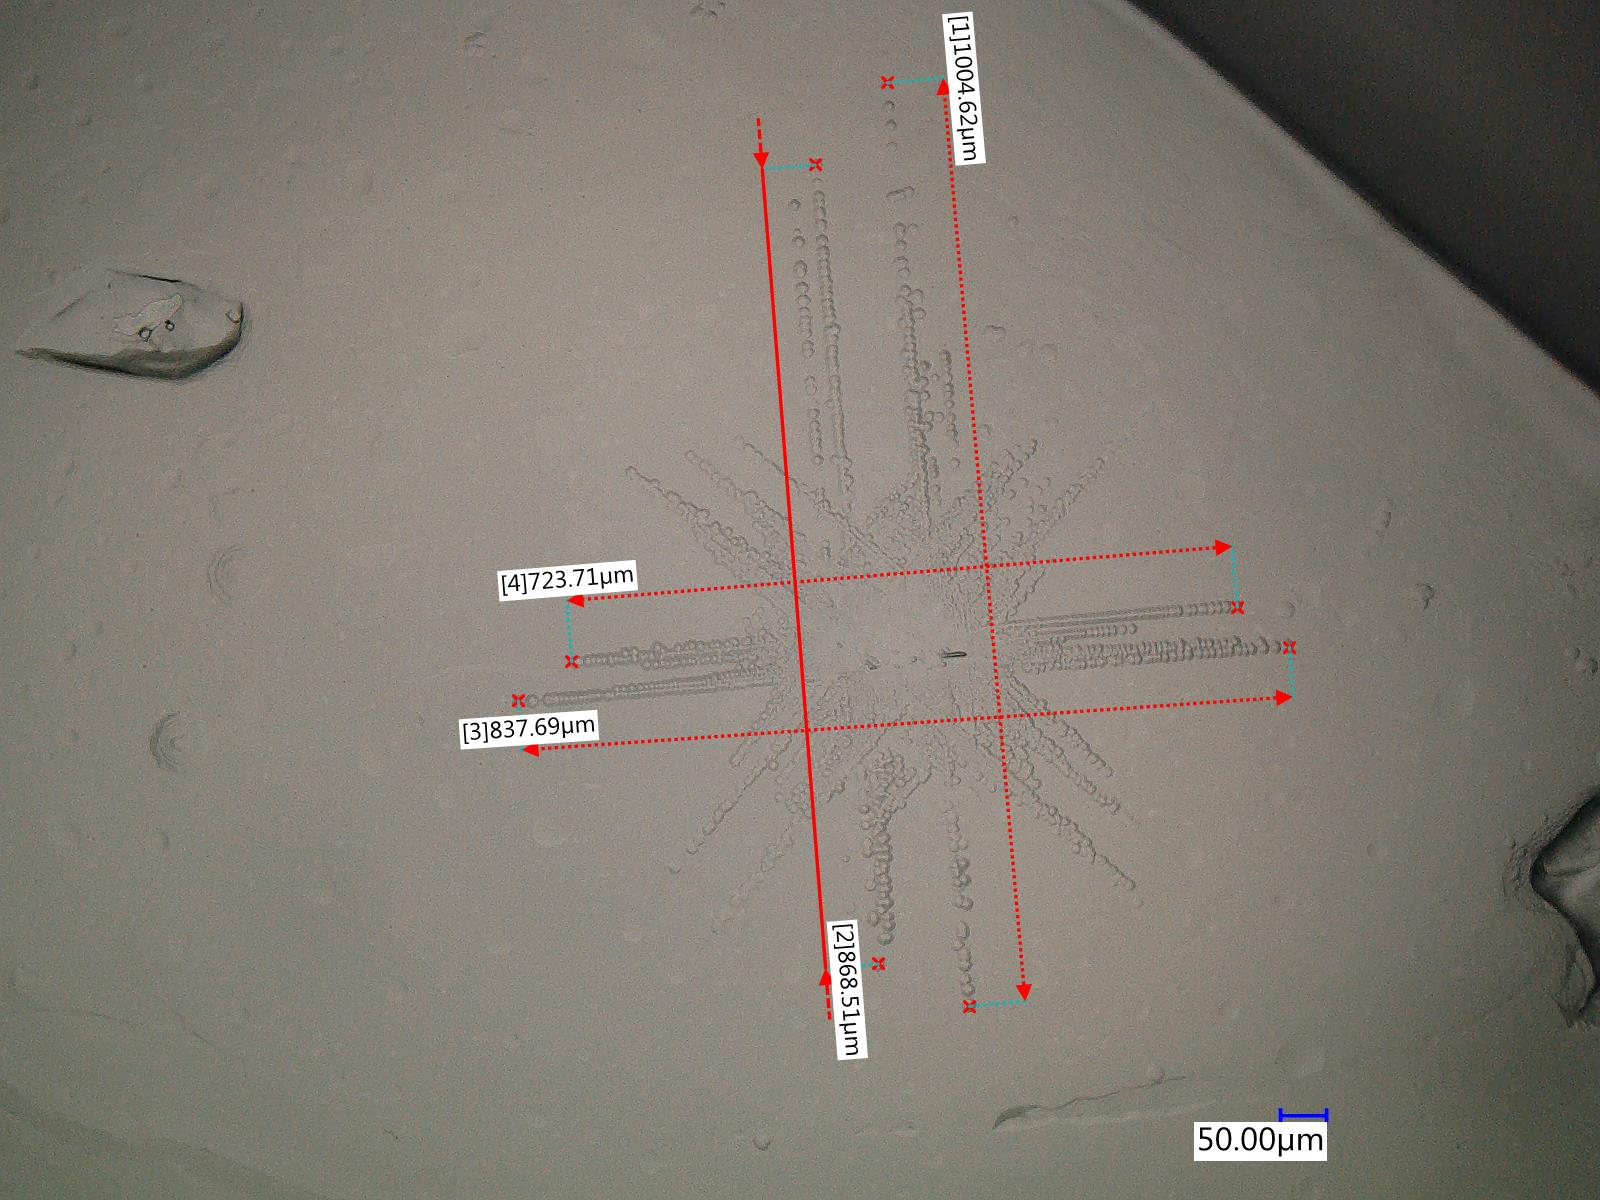
\includegraphics[width=\linewidth]{Images/eriks rosette 1 messung A.jpg}
                \end{minipage}
                \hspace{.1\linewidth}% Abstand zwischen Bilder
                \begin{minipage}[b]{.4\linewidth} % [b] => Ausrichtung an \caption
                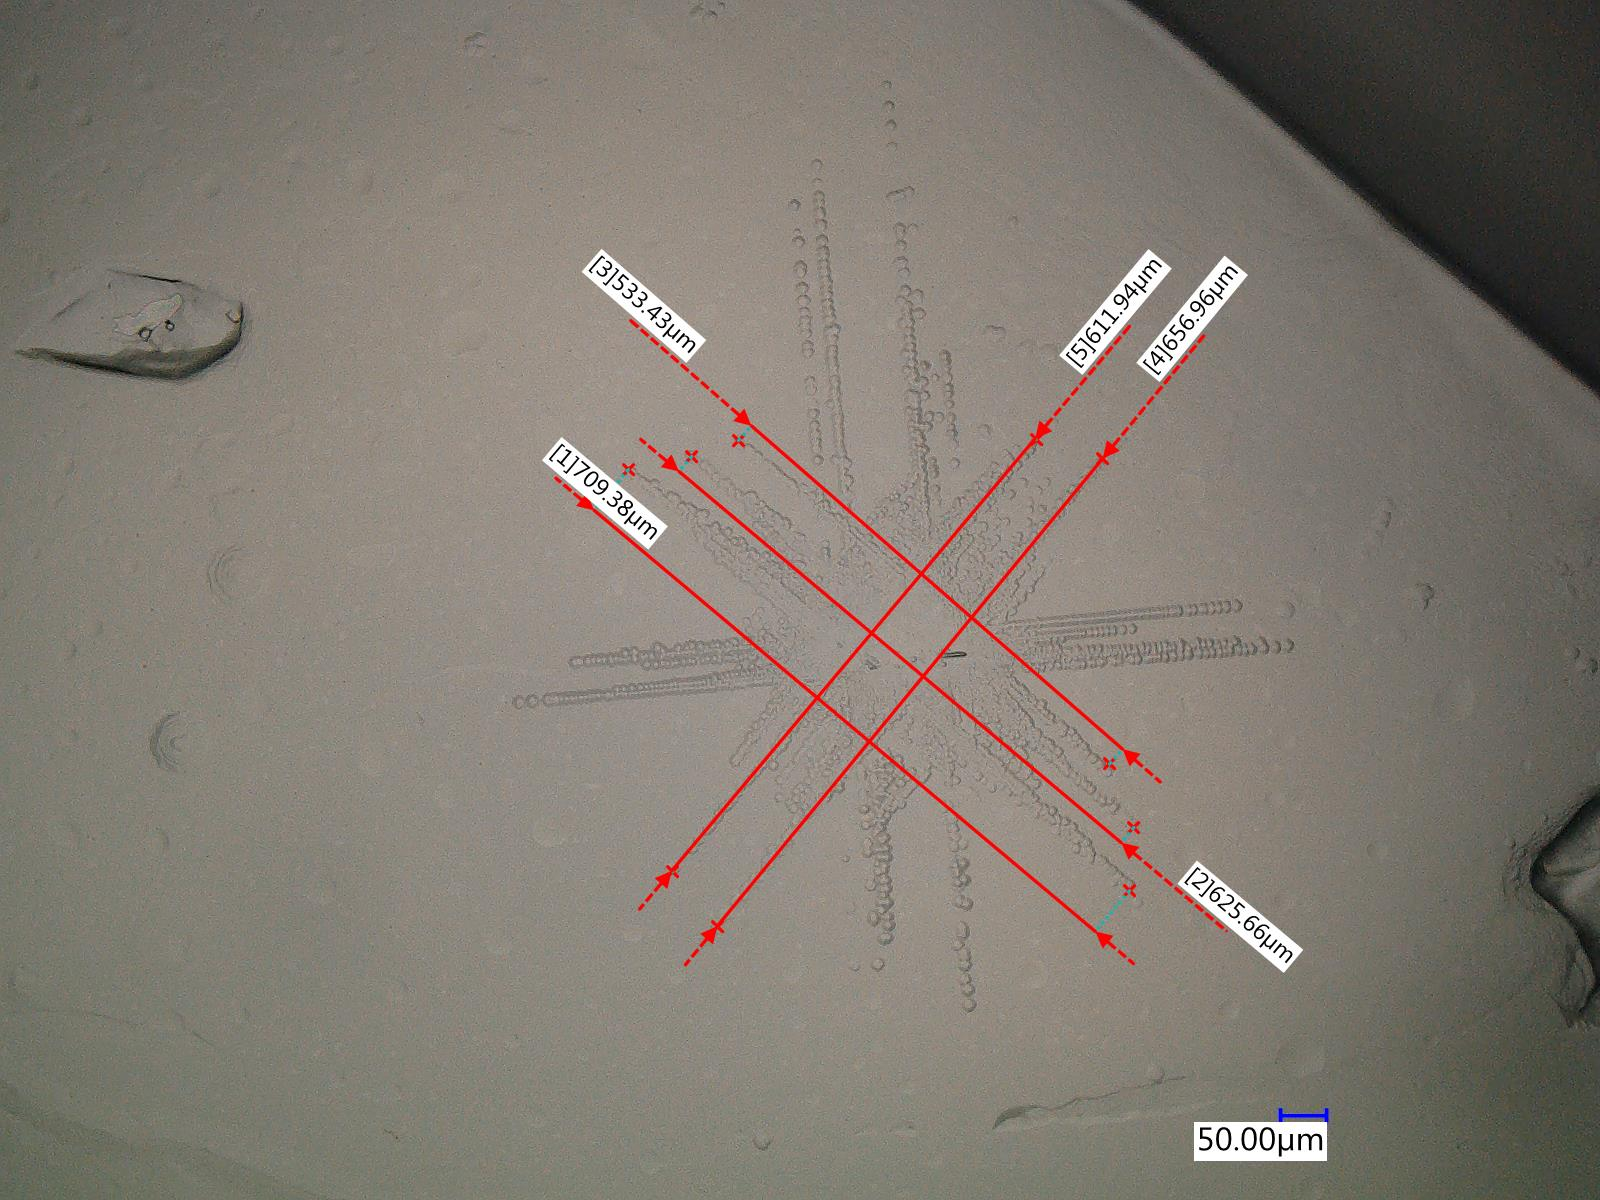
\includegraphics[width=\linewidth]{Images/eriks rosette 1 messung B.jpg}
                \end{minipage}
                \caption{Aufnahme eines Nadeleindrucks mit Abmessungen vor der Anwendung des Axialen Drucks}
            \end{figure}
            \begin{figure}[H]
                \centering
                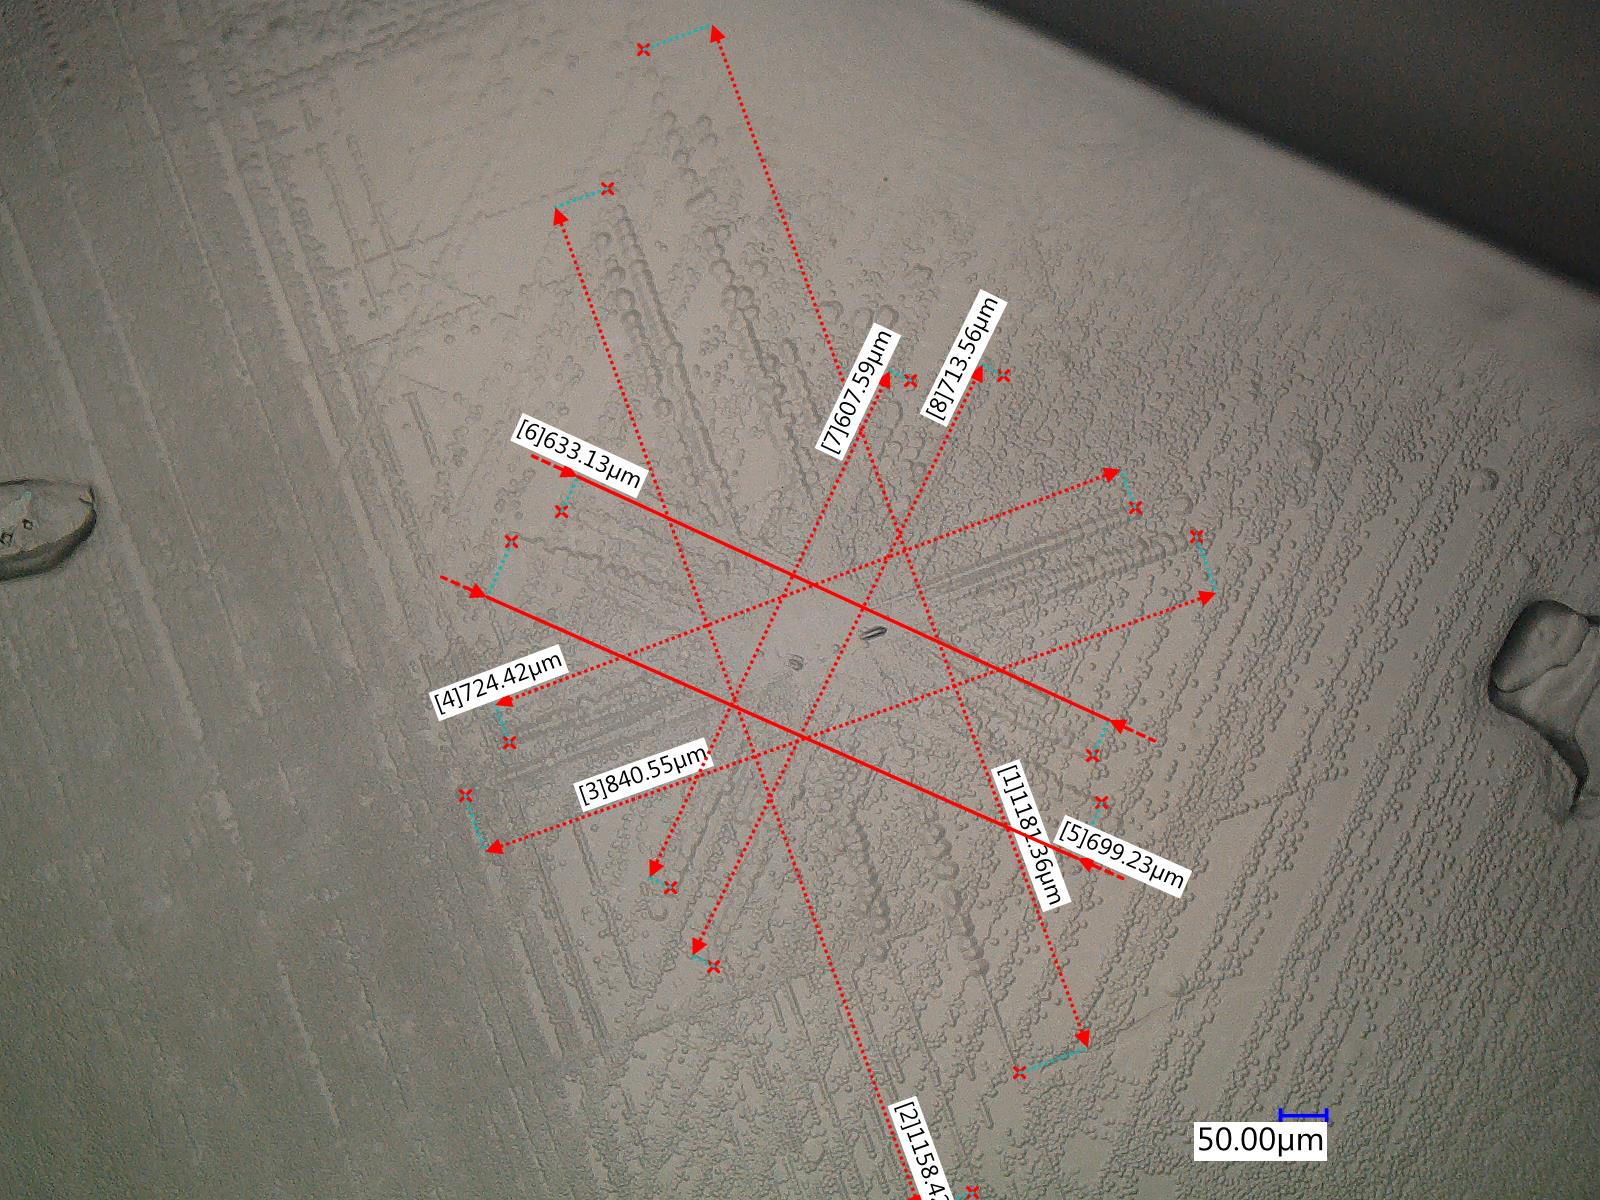
\includegraphics[width=\linewidth]{Images/eriks rosette 1PD Messung.jpg}
                \caption{Aufnahme eines Nadeleindrucks mit Abmessungen nach der Anwendung des Axialen Drucks}
            \end{figure}
            Aus den Messungen durch das Mikroskop lassen sich grob folgende Messungen für die Wanderungsdistanz bestimmen
            \begin{table}[H]
                \centering
                \begin{tabular}[]{c|c|c|c}
                    Vorher [$\mu m$] & Nachher [$\mu m$] & Differenz [$\mu m$] & Geschwindigkeit [$\frac{\mu m}{min}$] \\
                    \hline
                    $838 \pm 5$  & $841 \pm 5$    & $ 3 \pm 10$     & $1,0 \pm 3,3$ \\
                    $724 \pm 5$  & $724 \pm 5$    & $ 1 \pm 10$    & $0,2 \pm 3,3$ \\
                    $869 \pm 5$  & $1158 \pm 5$   & $ 290 \pm 10$  & $96,6 \pm 8,7$\\
                    $1005 \pm 5$ & $1181 \pm 5$   & $ 177 \pm 10$  & $58,9 \pm 5,9$\\
                    $533 \pm 5$  & $633 \pm 5$    & $ 100 \pm 10$    & $33,2 \pm 4,3$\\
                    $709 \pm 5$  & $699 \pm 5$    & $ -10 \pm 10$  & $-3,4 \pm 3,4$\\
                    $612 \pm 5$  & $608 \pm 5$    & $ -4 \pm 10$   & $-1,5 \pm 3,3$\\
                    $657  \pm 5$ & $714  \pm 5$   & $ 57 \pm 10$    & $18,9 \pm 3,7$\\
                \end{tabular}
                \caption{Messung der Wanderung der Rosettenarme}
            \end{table}
            Es ist deutlich zu erkennen, dass durch den axialen Druck nur wenige Arme entlang der $<110>$ - Richtung ein Starkes Wachstum erfahren haben, das Wachstum der anderen Arme ist im Rahmen unserer
            Messgenauigkeit kaum aussagekräftig, ließe sich jedoch auf die statistische Verteilung der Energie entlang aller Achsen zurückführen.
		Das ausbleibende Wachstum der Arme in $<100>$ - Richtung entspricht grundsätzlich unseren Erwartungen, wir hätten allerdings auch ein deutlicher sichtbares Wachstum der Arme in $<110>$ - Richtung erwartet.
		Vermutlich hätte sich durch ein höheres Lastgewicht oder eine erhöhte Belastungsdauer ein stärkeres Wachstum ergeben. Genauso hätte dies jedoch auch eine Zunahme der Fehlstellen abseits der Nadeleindrücke
		verursachen können, was die Auswertung an dieser Stelle erschwert hätte. Bereits in unserer Aufnahme ist zu erkennen, dass sich durch die Belastung unzählige zusätzliche Fehlstellen auf der Kristalloberfläche
		gebildet haben.
        \subsubsection*{Schubspannung im Gleitsystem}
            Um den Druck im Gleitsystem zu bestimmen wurde das angewandte Gewicht ($m = 2,716\pm0,01\text{ Kg}$) der Presse sowie die Druckfläche ($A=3618962\text{ }\mu m^2$)der Probe bestimmt.
            Mit
            \begin{equation}
                F = m \cdot a = 26,64\pm0,10\text{ N}
            \end{equation}
            folgt die Kraft (Fehler: 0,01 Kg$\cdot$9,81 m/s$^2 \approx$ 0,10). Die Kraft entlang der bevorzugten 
            gleitebene berechnet sich mit der Gitterkonstante a=0.402 nm zu\cite{7} 
            \begin{equation}
                F_{<110>} = F\cdot b_{<110>}^2 = \frac{a^2}{2} \cdot F 
            \end{equation}
            und anschließend die über
            \begin{equation}
                \sigma = F_{<110>} \cos{(\pi / 4)}/ A = (4,2 \pm 0,016)\cdot 10^{-13}\text{ }\frac{N}{m}
            \end{equation}
            die Schubspannung. Der Fehler ergibt sich unter der Annahme, dass unsere Auswahl der Messpunkte im Auswertungsprogramm des Mikroskops eine lineare Ungenauigkeit von 1$\mu$m (und somit einen Flächenfehler von (1$\mu$m)$^2$) aufweist, mittels Fehlerfortpflanzung aus $\Delta \sigma^2 = (\frac{\cos{(\pi / 4)} \Delta F_{<110>}}{A})^2 + ( \frac{\cos{(\pi / 4)} F_{<110>} \Delta A}{A^2})^2$.